
\documentclass[twocolumn]{revtex4-1}
\usepackage[]{graphicx}
\usepackage{float} 
\renewcommand{\figurename}{graph}
\begin{document}

\title{
Software Final Write-up
}

\author{M.~Bellis}
\author{Kristin Ludwicki}
\affiliation{Siena College, Loudonville, NY}

\date{\today}

\begin{abstract}
    The goal of our Software for Physicists final project was to determine whether or not a person could escape a velociraptor.
Given that a velociraptor's velocity is 18m/s, a person's velocity is 3 m/s with a 30 meter head start, and acceleration= 0, we calculated the time and position in which the raptor would catch the person, the time and position in which the raptor was 1 meter behind the person, and the probability a person could escape the raptor. 
\end{abstract}

\maketitle{

\section {Explanation of Algorithms} 
I first created a position vs. time graph for both the velociraptor and the person using velocity as slope and initial position as the starting point on the y-axis. I plotted the equations $y=3x + 30$ for the person and $y1=18x$ for the velociraptor using matplotlib and numpy. In order to calculate when and where the velociraptor catches the person I used a while loop starting at time=0 and ending at time=5. The while loop calculated all the positions at times between 0 and 5 for the functions above and found when the position of the velociraptor equaled the position of the person. I used this same approach to calculate when the times of the two functions were equal to find that the velociraptor would catch the person at 36 meters in 2 seconds. This approach could also be solved algebraically by setting the two equations equal to each other and solving for x when asked for time and solving  for y when asked for position. Doing this procedure with coding or with pen and paper produces the same answers. In order to calculate the position and time when the velociraptor was 1 meter behind the person I subtracted 1 from the velociraptors position and manipulated both functions to solve for time. Then I looped through distances from 30 to 60 in steps of .01 to find the moment when the raptors time was just under the person's time. I used the same approach to find time by manipulating the functions accordingly. Though this method I found that the person ran 35.82 meters and 1.9367 seconds when the raptor is one meter away from the person. This could also be done algebraically by setting the position minus 1 equal to the person's equation. Then I solved for x when asked for time and y when asked for position. When solving for both values on pen and paper, the numbers were off by about .01: the position was 35.80 and the time was 1.933. Lastly, I solved for the probability that a person could escape the velociraptor by creating a function which took random numbers and used them to evaluate how many times that number was less was 20, 15, or 7 percent. Then, I made that same function loop through that function 1000 times and tallied how many times the velociraptor succeeded or failed. The amount of tallied successes was then divided by 1000, the number of attempts, and then multiplied that number by 100 to come up with a probability that a person could escape. Though this technique I found that the person has about a 61 percent chance of escaping. 

\section{Position vs. Time Graph}
\begin{figure} [H] 
    \centering
    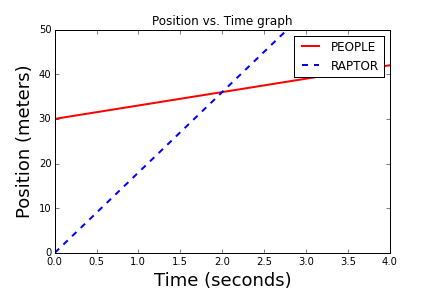
\includegraphics[width=0.5\textwidth]{graph.png}
    \caption{This is the position vs. time graph.\label{fig:graph}}
\end{figure}

\section{Equations used:}

I used the formula $y=mx+b$ to figure out the position vs. time plot for both the velociraptor and the person. I set these two equations equal to each other and solved for x to find time:
$$y=3x+30$$
$$y1=18x$$

To solve for position, I manipulated the equations to solve for y:
$$x=(y-30)/3$$
$$x1=y/18$$

To solve for how long the person ran when the velociraptor was one meter behind him I subtracted 1 from the the velociraptors position y1, set it equal to the person's equation, and solved for x:
$$y=18x+1$$
$$y=3x+30$$

To solve for how far the person ran when the velociraptor was one meter behind him I also subtracted 1 from the the velociraptors position y, set the functions equal to each other, and solved for x:
$$x1=(y-1)/18$$
$$x=y-30/30$$

To find the chance that the person could escape the velociraptor I used the equation:
$$chance= (amount of successes/total time) 100$$



\end{document}

